\documentclass[conference]{IEEEtran}
\IEEEoverridecommandlockouts
% The preceding line is only needed to identify funding in the first footnote. If that is unneeded, please comment it out.
\usepackage{cite}
\usepackage[ngerman]{babel}
\usepackage[utf8]{inputenc}
\usepackage{amsmath,amssymb,amsfonts}
\usepackage{algorithmic}
\usepackage{graphicx}
\usepackage{textcomp}
\usepackage{xcolor}
\usepackage{listings}


\definecolor{pblue}{rgb}{0.13,0.13,1}
\definecolor{pgreen}{rgb}{0,0.5,0}
\definecolor{pred}{rgb}{0.9,0,0}
\definecolor{pgrey}{rgb}{0.46,0.45,0.48}
\lstset{language=Java,
	showspaces=false,
	showtabs=false,
	breaklines=true,
	tabsize=2,
	showstringspaces=false,
	breakatwhitespace=true,
	commentstyle=\color{pgreen},
	keywordstyle=\color{pblue},
	stringstyle=\color{pred},
	basicstyle=\ttfamily
}


\usepackage{url}
\def\BibTeX{{\rm B\kern-.05em{\sc i\kern-.025em b}\kern-.08em
		T\kern-.1667em\lower.7ex\hbox{E}\kern-.125emX}}
\begin{document}
	
	\title{Computational Geometry - Abgabe 4}
	
	\author{\IEEEauthorblockN{1\textsuperscript{st} Bartolovic Eduard}
		\IEEEauthorblockA{\textit{Hochschule München} \\
			München, Deutschland \\
			eduard.bartolovic0@hm.edu}
	}
	
	\maketitle
	
	
%\begin{abstract}	
%\end{abstract}

	\section{Konvexe Hülle}
	Für die Berechnung der Konvexe Hülle wurde das Programm \textit{qhull} \cite{b2} verwendet. \textit{qhull} verwendet den Quickhull Algorithmus um die Konvexe Hülle zu berechnen. \textit{qhull} lässt sich per Kommandozeile ansprechen. Ein Beispiels für einen Aufruf:
	\begin{lstlisting}[basicstyle=\tiny]
	rbox 3 D2 | qconvex s o TO result
	\end{lstlisting}
	Der Befehl \textit{rbox} generiert eine gewisse Anzahl an Punkten in einer definierten Dimension. Der Befehl \textit{qconvex} berechnet die Konvexe Hülle. Mit einer Pipe können die Punkte direkt \textit{qconvex} übergeben werden.\\
	Es wurden verschiedene Untersuchungen durchgeführt.\\
	
	
	++++++++++++
	1 Punkt mehr als Dimensionen nötig
	+++++++

	\textbf{Laufzeit von \textit{qhull}}
	Es wurde die Laufzeit von \textit{qhull} untersucht. Hierbei wurden verschiedene Konfiguration bezüglich Anzahl und Dimension getestet. Um den Einfluss von Ausreißern zu reduzieren wurde das mittel aus fünf Durchläufen gebildet.\\
	Die Ergebnisse sind in den beiden Abbildungen \ref{figure_1} und \ref{figure_2} zu sehen.
	\begin{figure}[h]
		\begin{center}
			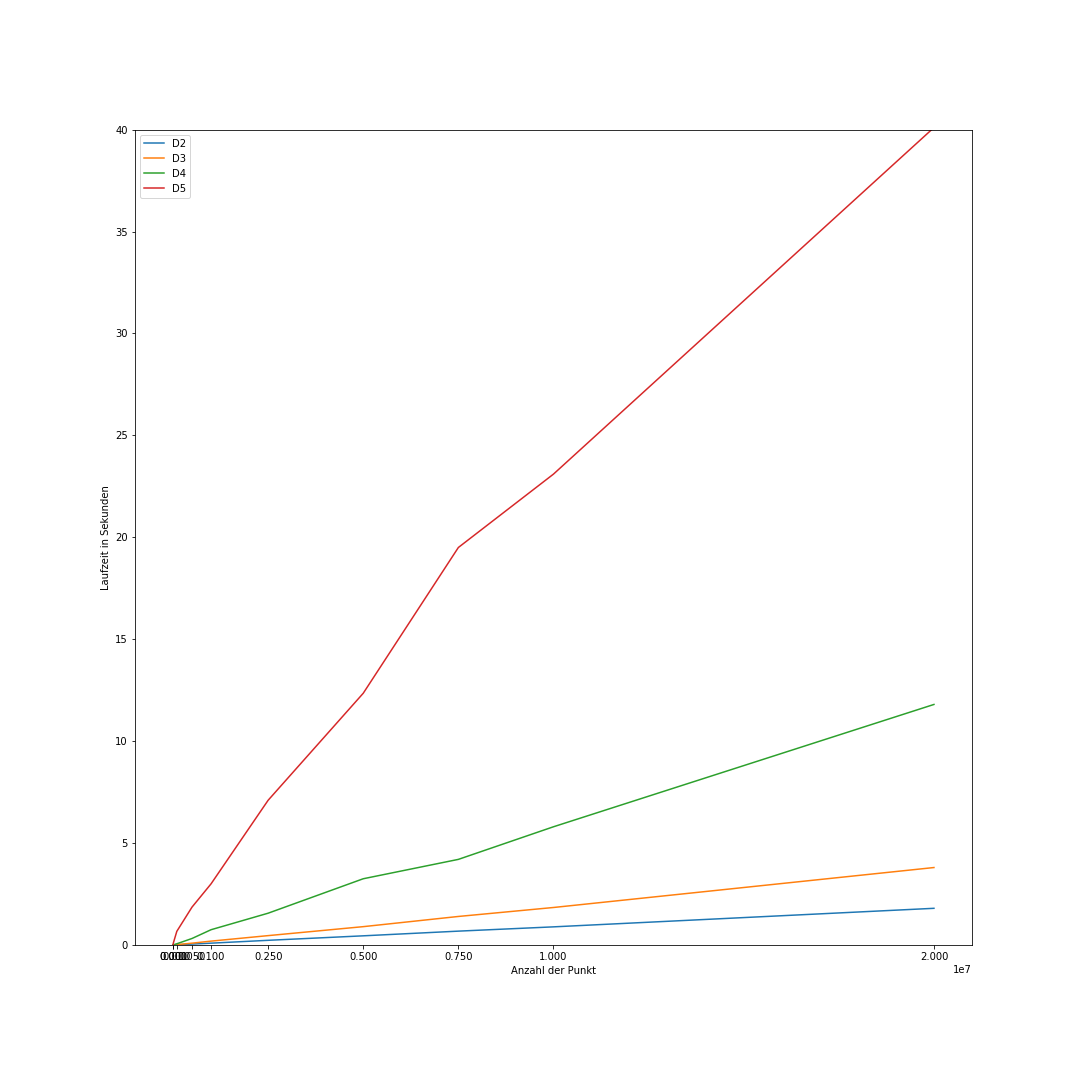
\includegraphics[width=7cm]{index.png}
			\caption{Messung der Laufzeit abhängig zur Anzahl der Punkte und Dimensionen}
			\label{figure_1}
		\end{center}
	\end{figure}
	\begin{figure}[h]
		\begin{center}
			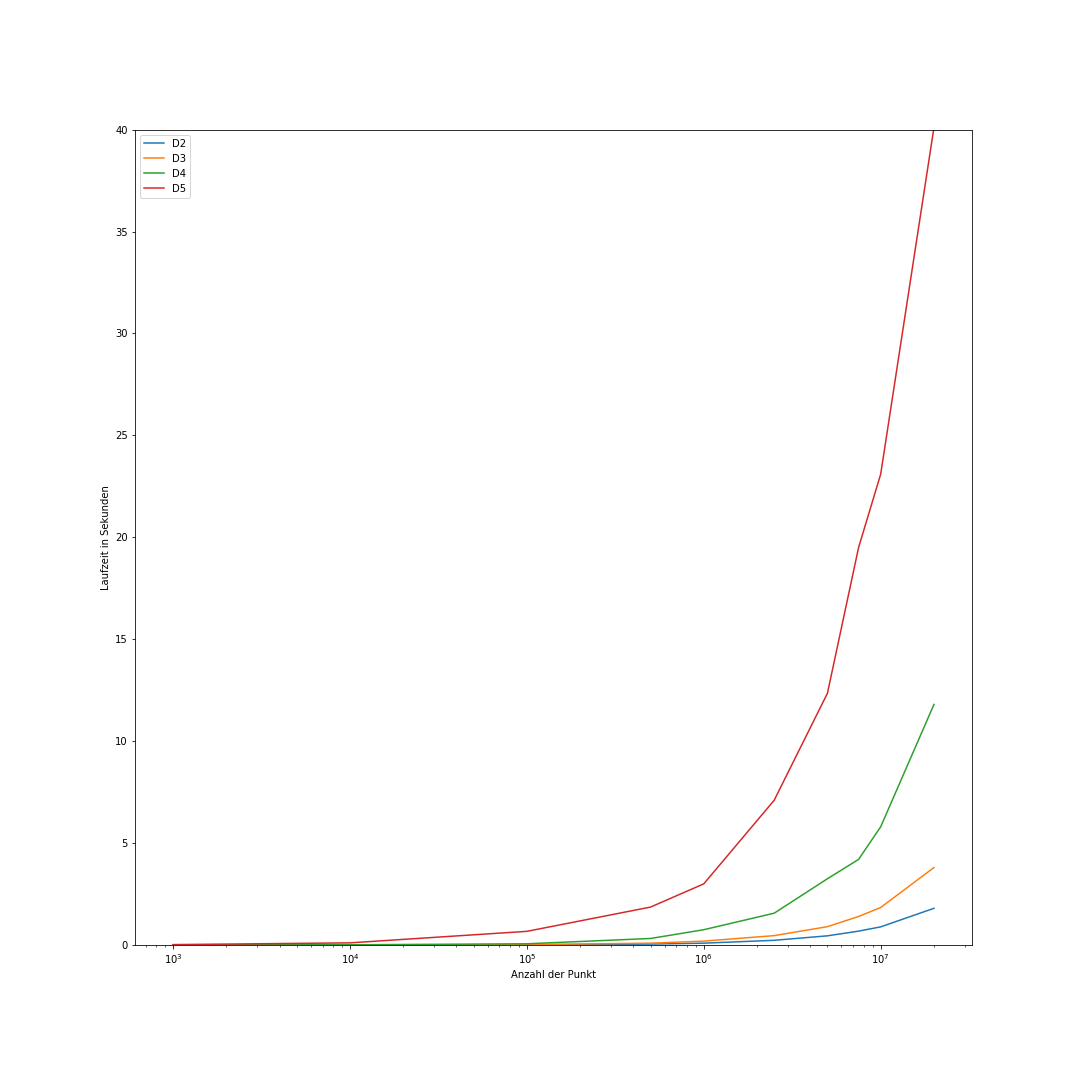
\includegraphics[width=7cm]{index2.png}
			\caption{Messung der Laufzeit abhängig zur Anzahl der Punkte und Dimensionen (X-Achse ist Log Skalierung)}
			\label{figure_2}
		\end{center}
	\end{figure}\\
	Wie gut in den Messungen zu sehen ist steigt der Aufwand mit Anzahl der Punkte und Dimensionen.
	Die gemessenen Laufzeitsteigerungen entsprechen grob der Komplexität $\mathcal{O}(n * \log(n))$???????.\\
	Dies entspricht auch dem Best Case Szenario von Quickhull. 
	Quickhull nutzt einen Divide and Conquer Ansatz um das Problem zu lösen. Im Zwei- und Dreidimensionalen besitzt das Verfahren eine Komplexität von $\mathcal{O}(n * \log(r))$ wobei n die Anzahl der Input Punkten entspricht und r die Anzahl der betrachteten Punkte.
	Im Zweidimensionalen hat Quickhull im Durchschnitt eine Komplexität bei zufälligen Punkten von $\mathcal{O}(n * \log(n))$.\\


+++++
N*logN Quickhull mit Worstcase $n^2$

Höher: 

Eine symmetrische Anordnung der Punkte besitzt jedoch eine höhere Wahrscheinlichkeit die Best Case (bester Fall) Laufzeitschranke von $\mathcal{O}(n * \log(n))$ zu verlassen und deutlich langsamer zu sein.
 
%Quickhull is a method of computing the convex hull of a finite set of points in n-dimensional %space. It uses a divide and conquer approach similar to that of quicksort, from which its name %derives. Its worst case complexity for 2-dimensional and 3-dimensional space is considered to be %O ( n log ⁡ ( r ) ), where n %{\displaystyle n} n is the number of input points and r {\displaystyle r} r is the number of %processed points.[1] However, unlike quicksort, there is no obvious way to convert quickhull %into a randomized algorithm. Nevertheless, there exist works from Smoothed Analysis which tell %us that the 2-dimensional Quick hull algorithm has expected runtime O ( n log ⁡ ( n ) ) %{\displaystyle O(n\log(n))} O(n\log(n))
	
	
	\begin{thebibliography}{00}
		\bibitem{b2} http://www.qhull.org/html/qconvex.htm
	\end{thebibliography}
	
	
	
	\section{Anhang}

	Batchfile zum Testen der Laufzeit von Q-Hull:
	\begin{lstlisting}[basicstyle=\tiny]
	rbox 5000000 D2 | qconvex s o TO result
	rbox 5000000 D2 | qconvex s o TO result
	rbox 5000000 D2 | qconvex s o TO result
	rbox 5000000 D2 | qconvex s o TO result
	rbox 5000000 D2 | qconvex s o TO result
	rbox 5000000 D2 | qconvex s o TO result
	rbox 5000000 D2 | qconvex s o TO result
	rbox 5000000 D2 | qconvex s o TO result
	rbox 5000000 D2 | qconvex s o TO result
	rbox 5000000 D2 | qconvex s o TO result
	\end{lstlisting}	

\end{document}
